\documentclass[twoside, 12pt]{article}
\usepackage[utf8]{inputenc}
\usepackage[default]{lato}
\usepackage{color,amssymb,amsmath,mathtools, enumitem} 
\usepackage{fullpage,caption, listings,clrscode,placeins, textcomp} 
\usepackage{setspace, sectsty}
\usepackage[all]{nowidow}

% Document settings
\pretolerance=10000
\tolerance=2000 
\emergencystretch=10pt
 % Metadata info
\newcommand{\mytitle}{HackPSU Technology Director Documentation} 
\newcommand{\mydate}{\today} 
\newcommand{\myauthors}{HackPSU Technology Team}

% Setting Hyperref parameters
\usepackage[
	bookmarks,
	bookmarksnumbered,
	citecolor={blue},
	pdfpagemode={UseOutlines},
	plainpages=false,
	pdfpagelabels=true,
	pdfauthor={\myauthors},
	pdftitle={\mytitle},
	pagebackref=true,
	pdftex,
	colorlinks=true,
	linkcolor=black,
	urlcolor={blue},
	pagebackref=true]
	{hyperref}
	
% Colors
\definecolor{commentgreen}{RGB}{2,112,10}
\definecolor{eminence}{RGB}{108,48,130}
\definecolor{weborange}{RGB}{255,165,0}
\definecolor{frenchplum}{RGB}{129,20,83}
\definecolor{hackpsuorange}{RGB}{214,118,85}
\definecolor{hackpsudarkblue}{rgb}{0.098,0.196,0.275}
\definecolor{hackpsulightblue}{rgb}{0.482,0.651,0.694}
\definecolor{hackpsured}{RGB}{186,76,58}
\definecolor{hackpsumdblue}{RGB}{43,75,105}

\sectionfont{\color{hackpsudarkblue}}
\parttitlefont{\color{hackpsuorange}\fontsize{48pt}{1.5cm}\scshape}

% LST Listing formatting
\lstset {
    language=C++,
    frame=tb,
    tabsize=2,
    showstringspaces=false,
    numbers=left,
    upquote=true,
    commentstyle=\color{commentgreen},
    keywordstyle=\color{eminence},
    stringstyle=\color{frenchplum},
    basicstyle=\small\ttfamily, % basic font setting
    emph={int,char,double,float,unsigned,void,bool},
    emphstyle={\color{blue}},
    % keyword highlighting
    classoffset=0, % starting new class
    morekeywords={>,<,.,;,,,-,!,=,~},
    keywordstyle=\color{weborange},
}
	

\title{\mytitle}
\author{\myauthors}
\date{\mydate}

% Some useful commands from CVPR
\usepackage{xspace}
\makeatletter
\DeclareRobustCommand\onedot{\futurelet\@let@token\@onedot}
\def\@onedot{\ifx\@let@token.\else.\null\fi\xspace}
\def\eg{\emph{e.g}\onedot} \def\Eg{\emph{E.g}\onedot}
\def\ie{\emph{i.e}\onedot} \def\Ie{\emph{I.e}\onedot}
\def\cf{\emph{c.f}\onedot} \def\Cf{\emph{C.f}\onedot}
\def\etc{\emph{etc}\onedot} \def\vs{\emph{vs}\onedot}
\def\wrt{w.r.t\onedot} \def\dof{d.o.f\onedot}
\def\etal{\emph{et~al}\onedot}
\makeatother


\pagestyle{empty}
\usepackage{fancyref,fancyhdr}
%\usepackage[hmarginratio=1:1, top=2.0cm, bottom=5.0cm, left=1cm, right=1cm]{geometry}
\setlength{\headheight}{14pt}
\setlength{\headsep}{10pt}
\setlength{\footskip}{50pt}
\pagestyle{fancy}
\fancyhf{}
\fancyhf[HLE,HRO]{\footnotesize{\myauthors}}
\fancyhf[HLO,HRE]{\footnotesize{\mydate}}
\fancyhf[FLO,FRE]{\footnotesize{\mytitle}} 
\fancyhf[FLE,FRO]{\thepage}
\renewcommand{\footrulewidth}{0.5pt}

\usepackage[pdftex]{graphicx}
\DeclareGraphicsExtensions{.pdf,.png,.jpg,.eps}
\usepackage[numbers, sort&compress]{natbib}
\usepackage[senames,dvipsnames,svgnames,table]{xcolor}

\newenvironment{tightitemize} % Defines the tightitemize environment which modifies the itemize environment to be more compact
{\begin{itemize}\itemsep1pt \parskip0pt \parsep0pt}
{\end{itemize}\vspace{-\topsep}} 

\newlist{checklist}{itemize}{2}
\setlist[checklist]{label=$\square$}

% Some useful packages (look at booktabs for good looking tables)
\usepackage{subcaption,booktabs,placeins}

\begin{document}
\begin{titlepage}
\begin{figure}[h]
    \centering
    
\includegraphics[scale=0.6]{logo.png}
    \label{fig:logo}
\end{figure}
{ \fontsize{48pt}{5.5cm} \flushleft \bfseries \textbf{\color{hackpsudarkblue}Technology \color{hackpsuorange} Director}}\\ [0.5cm]
{ \fontsize{48pt}{5.5cm} \color{hackpsured} \textbf{Hack\color{hackpsumdblue}PSU} }\\ [0.5cm]
{ \Huge \textit{\color{hackpsulightblue}A Comprehensive Guide}}\\ [0.5cm]
\begin{minipage}{0.4\textwidth}
\large
\emph{\color{hackpsudarkblue}Authors:}\\
Sushrut \textsc{Shringarputale}\\ \textit{sush.shring@gmail.com}\\
Matthew \textsc{Heilman}\\ \textit{mdh5389@gmail.com}\\
\end{minipage}
\end{titlepage}

\tableofcontents
\newpage

\mbox{}
\vfill
\part{Introduction}
\newpage
\par Congratulations on your acceptance as Director of Technology! We're sure you were selected from a very competitive pool of applicants as the best choice for the role.
\par The Director of Technology has grown to be a very important role within HackPSU. A large portion of the success of the event hinges on the success of the tech team achieving their goals. Hence we believe that it is very important that you be prepared for anything the event may throw at you. 
\par This document will provide a high-level overview of the responsibilities of the Director of Technology for HackPSU. It lists the necessary information and tasks needed to make HackPSU a successful event as far as the Tech Team's contribution is concerned.
\par The next page lists a number of tasks that should help you keep a track of all the tasks needed to be completed before, during, and after the event. The rest of the document goes into considerable detail about the goals and responsibilities of the Tech Team and the Director.
\begin{figure} [ht]
  \centering
  \caption{Tech Projects}
  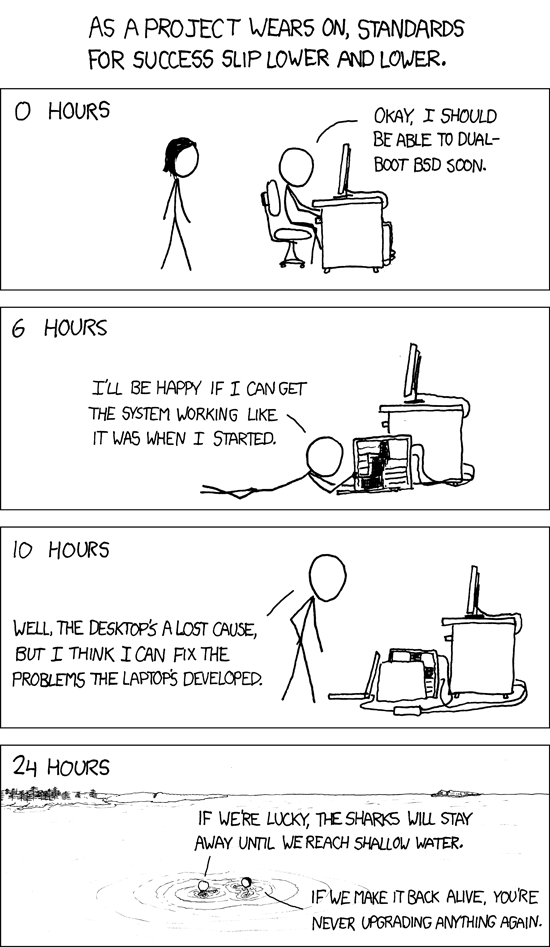
\includegraphics[width=0.45\textwidth]{success.png}
  \caption*{Source: \href{https://xkcd.com/349}{\textit{xkcd.com/349}} \cite{xkcd_success}}
  \label{fig:success}
\end{figure}
\newpage
\section{Checklist}
\par This page is a quick TL;DR of suggested tasks that need to be taken care of during the semester. This list is in no way comprehensive or mandatory, but it should give you a good sense of how to structure the semester. The list is formatted as \textit{[item - suggested time to complete]}
\paragraph{Pre-event}
\begin{checklist}
    \setlength\itemsep{1pt}
    \item Budget Proposal - 14 WBE \footnote{Weeks before event}
    \item Finalize Landing Page Design - 12 WBE
    \item Open Registration - 10 WBE
    \item Order RFID Bands - 5 WBE
    \item Synchronize Sponsors on website - Continuous process
    \item Finalize plan for live website and tracking system - 3 WBE
    \item Synchronize dietary restriction data with Logistics - 3 WBE
    \item Talk to PSU IT and boost building internet capacity - 2 WBE
    \item Generate day-of Slack - 1 WBE
    \item Send email to all registrants with pin number - 1 WBE
    \item Finalize and update schedule on the database - 1 WBE
    \item Finalize and update workshops on the website - 1 WBE
    \item Finalize and update prizes on the Website/Devpost - 1 WBE
    \item Update times for live countdown timer - 1 WBE
\end{checklist}
\paragraph{Week-of event}
\begin{checklist}
    \setlength\itemsep{1pt}
    \item Redirect hackpsu.org to the live website - 3 DBE
    \item Upgrade server and database capacity - 1 DBE
\end{checklist}
\paragraph{Post-event}
\begin{checklist}
    \setlength\itemsep{1pt}
    \item Downgrade server and database - 1 WAE \footnote{Weeks after event}
    \item Change landing page - 1 WAE
    \item Team Debrief - 1 WAE
    \item Change active hackathon on database - 2 WAE
\end{checklist}

\newpage
\section{Essentials}
\par Just the essentials that will help you succeed in your position. This should be a good enough reference for any information you may need during your term as director.
\subsection{Task Descriptions}
\subsubsection{Pre-event}
\begin{tightitemize}
    \item \textbf{Budget Proposal}
    \par One of the important tasks at the start of the semester is to come up with the budget for the Technology team. This budget needs to be submitted to the Finance team at the very start of the semester. The budget does not need to be extremely accurate, but should reflect a good enough estimate of the expenses of the semester. This helps the Finance team keep track of expenditure by each team. For reference, refer to old hackathon budgets.
    
    \item \textbf{Finalize Website Design}
    \par This does not mean that the whole design of the website be ready and coded up, but a general idea of what the website will end up looking like will help keep the Frontend project on track. Ideally, this task should be done in collaboration with the Design team.
    
    \item \textbf{Open Registration}
    \par This task is fairly straightforward. Test out that registration works properly for the current hackathon and open it up to the public.
    
    \item \textbf{Order RFID Bands}
    \par Order the RFID bands based on the current number of registrations. We recommend using manufacturers listed in section \ref{section:alibaba}. In case a design change is needed, order the bands further in advance as they may take extra time to confirm the design with the vendor. Another thing to keep in mind is the Chinese New Year which forces all factories to shutdown for about two weeks. This occurs around February and affects the Spring hackathon.
    
    \item \textbf{Synchronize Sponsors on website}
    \par Whenever sponsors are confirmed by the Sponsorship team, their logos should be added to the landing page. Depending on the tier, the logo size should vary.
    
    \item \textbf{Finalize plan for live website and tracking system}
    \par Decide what data will be displayed on the live website and start asking other teams for the data you will need to have a functional live website. Test and stress-test the tracking (RFID Scanner) system to ensure smooth check-in.  Some of the information needed includes workshop data, event schedule, prizes for challenges.
    
    \item \textbf{Synchronize dietary restriction data with Logistics}
    \par Logistics requires that they are provided an estimate of how many special meals to order for the event. We collect information about dietary restrictions (Halal, Kosher, Vegan, etc.) on the registration form, which should be shared with Logistics. The registration form should also note that any requests made after the 3 week mark will most likely not be fulfilled.
    
    \item \textbf{Generate day-of Slack}
    \par Sponsors and participants like having a day-of Slack to get updates, information, and help during the event. A link to this workspace should be made available on the live website and included in the email send to participants a week before the event.
    
    \item \textbf{Send email to all registrants with pin number}
    \par We send out an email to all registered participants containing their pin for registration. This email should also contain important event information like the schedule, workshops, and location. This email is an opportunity to remind hackers that they have registered for HackPSU and should come to the event. To send this email, craft up the HTML and use the Admin app's email send feature which generates emails unique to each hacker based on their information.  Registrations completed after the initial email is sent out should receive this email after they register.
    
    \item \textbf{Finalize and update schedule on the database}
    \par This is fairly straightforward as well. Use the admin app to update all the schedule information including event rooms, descriptions, and times in the database.  Make sure all the information is correct from the Education and Logistics teams.
    
    \item \textbf{Finalize and update workshops on the website}
    \par If the live website contains a section listing all the workshops separately from the event, it should be updated with location, time, and descriptions.  Make sure all information is correct from the Education team.
    
    \item \textbf{Finalize and update prizes on the website}
    \par A good way of listing out all the prizes for the hackathon is to link to Devpost and create the list of prizes there. This allows you to change the prizes whenever needed and also declare winners for them after the event easily.
    
    \item \textbf{Update times for live countdown timer}
    \par The live website timer has hardcoded Unix times for when the hackathon starts and ends. The constants in the code should be updated to refer to the new times for the hackathon. Keep daylight savings in mind if it becomes a factor.
\end{tightitemize}
\subsubsection{Day-of event}
\begin{tightitemize}
    \item \textbf{Upgrade server and database capacity}
    \par Remove any replication caps from the server to allow it to scale as needed for check-in and the rest of the event. Upgrade the database to use a larger machine and we recommend also creating a failover replica (Easily doable through the Google Cloud Console).
    
    \item \textbf{Talk to PSU IT and boost building internet capacity}
    \par PSU IT configures any special wireless networks we may need and also boosts the capacity of the PSU network in the building to be able to handle the nearly 1000 participants. Talk to Christy Long or IT directly to have this handled.
\end{tightitemize}
\subsubsection{Post-event}
\begin{tightitemize}
    \item \textbf{Downgrade server and database}
    \par Downgrade the server and database back to the original configuration to prevent unwarranted costs.
    
    \item \textbf{Change landing page}
    \par The landing page should be changed to a thank you page after the hackathon in preparation for the next event.
    
    \item \textbf{Team Debrief}
    \par We recommend going through a team debrief meeting in order to gauge what went well during the event and what should be worked on for next semester.
    
    \item \textbf{Change active hackathon on database}
    \par Once the hackathon is over, a Tech Admin (Refer to permissions in section \ref{section:api} should create a new hackathon entry and mark is as the next active hackathon. This step means that you have successfully executed everything necessary for the current hackathon. Congratulations!
\end{tightitemize}
\subsection{Accounts}
\par This section lists all the associated accounts that the Tech Team comes in contact with. The passwords for all the accesses to these accounts are available in encrypted form on Google Drive.

\subsubsection{Google Cloud Platform (GCP)}
\par 99\% of all server-side computing power is leased from GCP (with the exception of the local Redis server (eee section \ref{section:redis}). This account is perhaps the most important of all accounts. This includes the API servers, SQL Database, Email service, Realtime-Database service, Storage, and Authentication.
\par All Google related management is handled through the \textit{hackpsudev@gmail.com} account. We recommend using this account only for super admin \footnote{sudo} access. Google allows other users to be added as managers of projects with varying levels of access. 
\par GCP access is two-fold: Firebase and GCP itself.
\begin{tightitemize}
    \item Firebase:
    \par Firebase provides easy access to Identity and Access Management (IAM) (read authentication). The docs for Firebase can be found at \href{https://firebase.google.com}{\textit{firebase.google.com}} \cite{google_firebase}. Additionally, we use Firebase to host our landing page and realtime database.
    \begin{itemize}
        \item \textbf{IAM}
        \par For authentication, Firebase provides Single Sign On (SSO) \cite{esplin_2016} using secure OAuth protocol. Authentication is provided through simple email or via third parties such as Google, Facebook, and GitHub. \footnote{NOTE: We are not associated with Penn State authentication in any way. It is recommended that we inform hackers about this when registering to prevent them from using their Penn State email and password.}
        \item \textbf{Hosting}
        \par Our domain is purchased through Namecheap, but the landing page is hosted through Firebase. Namecheap simply redirects requests to \href{https://hackpsu.org}{\textit{hackpsu.org}} to Firebase. The benefit of using Firebase is the ease of use and the free SSL certificate that they provide to any website hosted there.
        \item \textbf{Realtime Database service}
        \par The Realtime Database is an interesting piece of technology that allows clients to subscribe to updates to the database. Any addition, change, or deletion from the database is pushed as an update to the clients subscribed to it. We use this to provide live updates during the event. The database is very scalable and extremely fast in pushing out updates. It also abstracts away all the difficulty in creating a "realtime messaging" system.
    \par Managing Firebase systems are handled through the Command Line Interface (CLI). Download it at \href{https://firebase.google.com/docs/cli/}{\textit{firebase.google.com/docs/cli}}
    \end{itemize}
    \item Gooogle Cloud Platform:
    \par All server-side computation is performed using the full Google Cloud suite (\href{https://console.cloud.google.com}{\textit{console.cloud.google.com}}). The following products from Google Cloud are in use by HackPSU currently:
    \begin{itemize}
        \item \textbf{App Engine}
        \par App Engine provides compute power as needed based on incoming demand. We use App Engine to run the API server (See section \ref{section:api}).
        \item \textbf{Cloud SQL}
        \par The main database used by HackPSU is hosted on Cloud SQL (See section \ref{section:database}).
        \item \textbf{Storage service}
        \par Any large files that need to be stored online are stored here. This includes resumes from registrations, reimbursement receipts, and anything else the server may need to upload.
        \item \textbf{Logging and Monitoring}
        \par While not exactly an active service used, StackDriver logging is one of the most important tools to ensuring that the server is functioning correctly. Debugging any issues on the backend should be directed here. This service keeps an eye of the responses that the server sends and aggregates any errors that may be occurring.
    \end{itemize}
    \begin{figure} [ht]
    \centering
    \caption{The Canonical Cloud}
    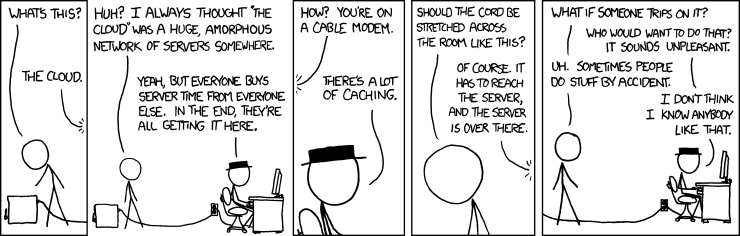
\includegraphics[width=0.8\textwidth]{the_cloud.png}
    \caption*{Source: \href{https://xkcd.com/908}{\textit{xkcd.com/908}} \cite{xkcd_success}}
    \label{fig:cloud}
    \end{figure}
\end{tightitemize}

\subsubsection{Amazon Web Services (AWS)}
\par The only use of AWS currently is for hosting the built and compiled web applications (admin app [Section \ref{section:admin}] and registration [Section \ref{section:registration}]). This is necessary because Google Cloud Storage does not support hosting with SSL and Firebase can only host one website per project.

\subsubsection{Namecheap}
\par All domain management is performed at \href{https://namecheap.com}{namecheap.com}. This includes hosting records for the main landing page, sub-domain pages, service verifiers (mainly email service), and email forwarders. You will have to renew both hackpsu.org and hackpsu.com\footnote{There was a push to deprecate the .com domain. Check with the exec team if this needs to be renewed any more.} domains each year.

\subsubsection{Github}
\par All of HackPSU's source code is up on Github. All the repositories are owned by the Hack-PSU organization, which you should be an admin for. The organization page is at \href{https://github.com/Hack-PSU}{github.com/Hack-PSU}. Most of the repositories on Github are integrated with Travis Continuous Integration (CI) (Section \ref{section:travis}).
\par Some notes on the repo structure:
\begin{tightitemize}
    \item The master branch of a repo should be protected and direct push to it should be prevented unless extremely necessary. This branch is where Travis should run its integration. Any code pushed to master should be production ready and depending on the CI configuration may be directly released to production. A separate development (\texttt{dev}) branch should be used to run all active development on.
    \item Build a habit of detailed information in commit messages. This helps track down changes and issues if they arise at any point.
    \item A healthy Git repository builds every new feature or change on a new branch, and each person works on a separate branch for that feature. Once the branch is good to go and ready to push into production code, it should be squashed into one commit to prevent the history of the production branch from becoming unreadable.
    \item A good idea is to make a release on all repositories for each event.  This helps keep a record of what was used at each hackathon and can be used as a way to show changes between events.
\end{tightitemize}

\subsubsection{Alibaba} \label{section:alibaba}
\par Since we started using an RFID tracking system we have continually needed to acquire RFID wristbands.  We have been doing so through Mrs. Jan Hu, a vendor on Alibaba.  Some things to keep in mind when using Alibaba:
\begin{tightitemize}
    \item These vendors are in China so there is a large time difference
    \item Vendors do not communicate well in English so be very specific in what you ask and in your responses.
    \item Save the invoice for reimbursement.  If possible try to get something after paying for the order to make the reimbursement process easier.
\end{tightitemize}

\subsubsection{OneSignal}
\par OneSignal is a free service that provides push notifications on the live website for HackPSU. Push notifications are supported on Android devices and PCs currently. There are two projects on OneSignal currently configured - production and development. Any test push notifications should be sent on the development project, which can be configured to any GCS hosted application easily.

\subsubsection{Asana}
\par Asana is a project management tool we use for tracking progress within HackPSU. The Technology Team follows Agile principles while targeting goals, so Asana is an excellent tool to use for that. We highly recommend heavy use of the portfolio and timeline feature of Asana.

\subsubsection{Travis CI} \label{section:travis}
\par Travis is a useful \cite{stamas_2017} tool for automating the build, test, and deployment cycle for applications. Whenever a commit is pushed to master, our current configuration of Travis builds the code as defined by the build process, runs the tests defined in the code, and deploys it to the appropriate source where it is hosted\footnote{Refer to the section on the individual projects below for specific hosting information.}. Travis is extremely simple \cite{dwyl} to learn and configure, but can perform very complex and powerful tasks in the automation process.

\subsubsection{Devpost}
\par Devpost (\href{https://devpost.com}{\textit{devpost.com}}) is an important piece of responsibility that the Tech Team is expected to handle. Each hackathon recognized by MLH is expected to have a new Devpost page that outlines the barebones of the hackathon, but more importantly, the prizes that are available for the event. Hackers expect to be able to submit their projects on Devpost, regardless of how the hackathon is performing project submissions and judging. Additionally, once the prizes have been declared, hackers expect that the projects that won be marked as such on Devpost. See \href{https://help.devpost.com}{\textit{help.devpost.com}} for more information on how to work with Devpost.

\newpage
\subsection{Team Structure}
\par The technology group is divided into four main teams: Frontend, Backend, RFID, and Admin App. The exact breakdown of each project is listed out in below sections.  See Part \ref{part:projects} for details about each team's projects.
\par In the past, we have had a project manager that helps keep each project on track for the hackathon. Depending on the experience level of the members in the team, there may be a mentor (project leader) that helps newer members get familiar with the codebase. This person should also take charge of the project in question and work with the PM to keep it on track. 
\par When selecting new members, it is important to take note of what skills the team needs to be successful, as well as judging the candidate by how much they are willing to learn. Learning is a crucial part of the HackPSU Tech experience, so this should be the cornerstone for any team member that is being added. Depending on what the demographics (school year, technical skill, available time, etc.) of the team are, we recommend looking for either fresher or more experienced students. This ensures that there is a good distribution of people that are willing to learn new things and take over in the coming semesters and team members that are excited to lead projects and have the technical skill-sets to make that happen.
\subsection{Important Resources}
\subsubsection{Christy Long (Advisor)}
\par Our current advisor is Christy Long. She is Director with Penn State IT, and a huge supporter of HackPSU. She has incredible contacts all across the board and in the past has helped us with mission crucial tasks such as implementing special Wi-Fi at the event for hardware, coordination with Penn State IT for any other requirements, reaching out to companies (Microsoft, Apple, Google) for sponsorship, and any other administrative hurdles that we may have needed to cross while building up HackPSU. She is an amazing person and an incredible resource.
\subsubsection{Owned Hardware}
\par Presently, the Tech team owns the following:
\begin{tightitemize}
    \item 1 - Soldering iron
    \item 6 - RFID tracking system boxes (and one development version)
    \item 1 - Rack-mount server
\end{tightitemize}
\subsubsection{Recommended Practices}
\par 
\begin{tightitemize}
    \item First GitHub commit
    \par When new team members are added, we recommend that they be asked to make a small change to a new branch. Their change should go through the full Pull-Request procedure and then the branch should be deleted without merging. This gives them a good understanding of how the code review process works.
    \item Attend one or more hackathons
    \par A very important experience for all team members is to attend one or more external hackathons. It provides team members with extremely important perspective about how other hackathons are run. It also acts as a means of generating ideas for new things we may want to implement for HackPSU.
\end{tightitemize}

\newpage
\mbox{}
\vfill
\part{Projects} \label{part:projects}
\newpage
\section{Frontend} \label{section:registration}
\par The Frontend team is tasked with executing the design vision for HackPSU's online presence for the semester. This consists of two pieces - Landing page and Live website/registration application \cite{frontend_repo}. 
\subsection{Overview}
\subsubsection{Landing page}
\par The landing page is where \href{https://hackpsu.org}{\textit{hackpsu.org}} redirects to. It is build using plain HTML, SCSS, and JavaScript. The aim of the landing page is to provide the relevant information to anyone looking at HackPSU. The following information generally belongs on the landing page:
\begin{tightitemize}
    \item Event Date and Location
    \item Link to registration
    \item Link to sponsorship packet
    \item FAQ and general event information
    \item Skeleton of schedule
    \item Sponsors
    \item Social media links
\end{tightitemize}
\paragraph{Hosting}
\par The landing page is hosted using Firebase. As Firebase provides free SSL certificates, this provides us the ability to access hackpsu.org using the https protocol and a modicum of security. 
\par Since we use SCSS for the styling of the landing page, it must be compiled before it is uploaded to hosting.

\subsubsection{Registration App / Live Page}
\par We implemented a web-application for registration and the live page. This application is build using Angular \cite{angular_docs} as it requires heavy interaction with our backend and the user. Most features on this applications are protected by user authentication and are fairly customized to the user's information. As portions of this application have user-specific information, the following features were also implemented here.
\begin{tightitemize}
    \item Travel reimbursement submission
    \item Project submission and table assignment
\end{tightitemize}
\paragraph{Registration App Content} 
\par MLH requires every attendee to agree with their legal statement so we include that requirement in the registration app.  Additionally, MLH requests the name of each person who attended as well as their email address, school they attend, and their phone number after the event is over.  
\paragraph{Live Page Content} 
\par The live website contains information pertinent to the day of the event. The information on this page is much more dynamic and loads data from the live update source, live schedule, and a timer that counts down to the end of the hackathon. The following information is generally presented on the live website:
\begin{tightitemize}
    \item Countdown Timer
    \item Link to Slack registration
    \item Live Updates
    \item Live Schedule
    \item List of workshops
    \item Other Day-of Information
\end{tightitemize}
\paragraph{Hosting}
\par The live website application is built using Angular and Webpack, which generates statically loadable, minified files. These files are hosted on AWS's CloudFront and \cite{amazon_cloudfront} S3 as they have support for SSL certificates on any number of hosts. Currently, there do not seem to be any issues with the CI for this, meaning all pushes to \texttt{master} are directly built and uploaded to S3.
\subsection{Known bugs}
\paragraph{Travis}
\par Current Firebase admin authentication has some issues where the authentication token for CI environments expires very quickly. As a result, the continuous integration cycle for the landing page is broken and requires manual deployment.
\paragraph{Form Sanitization}
\par The travel reimbursement form, table submission form, and to a much lesser extent the registration form face input sanitization issues, especially across different platforms. This may cause some submissions to get rejected by the backend. The backend returns a well structures message in the JSON response, but it may not always bubble all the way to the UI properly.
\subsection{Future features}
\paragraph{Profile Page}
\par A much needed feature for the registration application is a profile page that allows the user to view and edit information about their registration. Currently the only way to do so is by emailing the HackPSU team directly and the changes being made directly to the database.
\paragraph{Extra Credit Registration}
\par Another useful to have feature would be providing hackers the ability to register for extra credit directly on the profile page. This would reduce a step during check-in and make it easier to manage.
\paragraph{Medium Integration on Landing page}
\par A proof of concept for this feature already exists as a pull request on the repo. This feature request was made by the Communications team. They would like us to feature recent posts from the HackPSU Medium account on the landing page in order to drive traffic to the blog.

\newpage
\section{Backend} \label{section:api}
\par The backend for HackPSU drives all the data and interfaces across all applications. It is written in JavaScript and is currently being migrated to TypeScript for better type-safety. The server runs on Node version 8+. A secondary server built on top of Redis is  used locally during the event, and acts as a write-through cache for the hardware deployed in the venue. This redundancy is created to ensure that in case of network failures, the scanners continue to function with no issues.
\subsection{Main Database} \label{section:database}
\par As explained above, the "Main Database Server" runs on Node v8+ and is deployed on Google Cloud's App Engine platform. The database backing the server is MySQL 5.6 which is deployed on Google Cloud's SQL service. The server is built as a RESTful service to provide sanitized access to the SQL Database.
\subsubsection{Overview}
\par The server processes HTTP requests from clients and provides them with data as requested. The server handles many parts of the various applications, and so it is required that it provide strong authentication, authorization, and encryption guarantees. To fulfill these, all requests to and from the server are encrypted using SSL over HTTPS. Any data access that is user specific requires the request to be made from an authenticated client with the proper permissions. The permissions model is explained below. Authentication and authorization support is provided by Firebase's Auth API, which integrates very well with all the front facing applications.
\paragraph{Permissions Model}
\par Permissions are broken into five categories as listed below:
\begin{tightitemize}
    \item \textbf{No permissions/Participant} - Participants have the least permissions. They are allowed to submit any forms found on the registration app, read live updates, and read schedule information. They have the permission to change their information, but currently there is no support for that on the frontend.
    \item \textbf{Volunteer} - The next level of permission is a Volunteer. Volunteers are people that are helping organize the event day-of, but are not part of the team during the rest of the semester. They have access to the admin-app (Section \ref{section:admin} but cannot make any changes to any data.
    \item \textbf{Organizer} - Organizers are part of the team and have access to most features that will not completely affect the integrity of the data for the event.
    \item \textbf{Director} - Directors have almost full root access to make any changes to the data barring some database tables on whom the success of the event depends.
    \item \textbf{Tech Member} - Literally everything. Members of the tech team have full access to do anything they want to any data, anywhere. This permission level is the \texttt{sudo} of the HackPSU system, so it should not be handed lightly.
\end{tightitemize}
\subsubsection{Known bugs}
\paragraph{Type Confusion}
\par On some occasions, JavaScript's poor typing may face type issues with incoming data. However, in the current release of the server, these issues have been at an all time low. As the server continues to grow, these issues may grow again, which is why the migration to TypeScript has been suggested.
\subsubsection{Future features}
\paragraph{Analytics Engine}
\par Since there is an abundance of data available now, an interesting feature to implement would be an analytics engine that takes current hackathon data and provides insights for the teams to make informed decisions.
\paragraph{Anonymous Authentication}
\par In order to rapidly register people during registration drives, it may be useful to support creating anonymous accounts so that the person does not have to sign up for an account. This is implementable via Firebase but may need some backend restructuring.

\newpage
\subsection{Redis Database} \label{section:redis}
\par Part of the infrastructure for HackPSU is the Redis Server which helps IOT devices  (scanners) connected to our network to maintain low latency between the scanners and our backend server. It also provides redundancy for when the network cannot send messages to the server because of the 800+ users on our network during events. Having a caching system setup will protect the system from losing messages that need to occur and allow our scanners to continue servicing users well beyond massive failure of our backend system.
\paragraph{Redis Server}
\begin{tightitemize}
    \item Runs Node v10+
    \item Runs on Docker or NPM/Node v10
    \item Runs Redis to host the in-memory cache
    \item Runs MongoDB to host the Permissions for the different User types.
    \item Uses Express.js to connect to the main server using a RESTful API
\end{tightitemize}

\subsubsection{Overview}
\par The server processes HTTPS requests from scanner clients and forwards the data that they provide as a write-back cache. This is ok because all scanners will access the cache before the server and won’t need to confirm data written to the main server.
\par The server also provides Scanners with information through HTTPS using read-through cache. It allows the scanners to be updated with the latest user and location information.
\par The server handles many parts of the various applications, and so it is required that it provide strong authentication, authorization, and encryption guarantees. To fulfill these, all requests to and from the server are encrypted using SSL over HTTPS. Any data access that is user specific requires the request to be made from an authenticated client with the proper permissions. Since the server is on-premises, we had to self-sign the SSL certificates. To verify the authenticity of the server, we have hardcoded the fingerprint of the SSL certificate into each scanner to help it identify valid certificates.
\paragraph{Permissions}
\begin{tightitemize}
    \item Scanner API Key: Give’s scanners access to the Redis server through HTTPS. It uniquely identifies each scanner and allows us to track which device is accessing what functions.
    \item Admin: Complete access to all features.
\end{tightitemize}
\subsubsection{Known bugs}
\subsubsection{Future features}
\begin{tightitemize}
    \item Setup Redis server to handle 100+ requests per second
    \item Have smart caching procedures implemented
    \item Implement API to allow scanners to run future features from Admin app and Main Server API
\end{tightitemize}
\newpage
\section{RFID Scanners}
\subsection{Overview}
\par This project is responsible for developing and maintaining each of the RFID scanners we are using to track attendance data.  Currently, there are 6 functional enclosures.  The hardware used is a NodeMCU, a RC522 RFID scanner, a 16$\times$2 LCD display with an I\textsuperscript{2}C driver, and a 4$\times$4 keypad.  Each of these components are soldered directly to a 3cm$\times$5cm PCB board.
\subsection{Known bugs}
\paragraph{Hardware usage}
\par After much use, some of the boxes have developed poor connections at the micro USB port.  Additionally, some of the LCD displays have been flickering due to use and had to be replaced.  
\paragraph{NodeMCU}
\par The current configuration leaves no free pins for future features.  Additionally, there were many development challenges slowing progress on this project.
\subsection{Future features}
\paragraph{Upgrading Circuitry}
\par The human aspect required to solder the connections was an unpleasant and imperfect process.  Creating a custom PCB for each enclosure will allow highly precise and consistent  results.  Adding this will also help other events who wish to adopt our system.
\paragraph{3D Printed Enclosure}
\par Having a 3D printed design will help the re-creation of a box be quicker and less difficult than manually assembling a box.  Additionally, not everybody has access to the tools required to make a wooden enclosure.
\paragraph{Sponsor Tracking System}
\par The thought behind this new system is to allow sponsors to keep track of who came to talk to them.  They can either use this as a means to track either how many people talked to them or specific hackers they are interested in receiving their resume.  Additionally, this should prevent people not attending the event from talking with sponsors until after they have checked in.  This should be considered if the circuitry is updated.
\paragraph{Additional Features}
\par Some smaller features that would be beneficial include:
\begin{tightitemize}
    \item item check-in/check-out
    \item allowing a hacker to be associated with a second wristband in case they lose the wristband they received from check-in
    \item displaying information about a hacker given a wristband
\end{tightitemize}


\newpage
\section{Admin App} \label{section:admin}
\par The Admin App is an internal tool that allows team members and directors to view and manage various parts of the current hackathon. It is currently live at \href{https://admin.hackpsu.org}{admin.hackpsu.org}.
\subsection{Overview}
\par The Admin App is written with the Angular framework in TypeScript. It is only accessible to team members and directors within HackPSU who need to be manually given access to the application. Authentication is again provided by Firebase.
\paragraph{Hosting}
\par Since the application is built using Angular, hosting it is possible using static, built files on Cloudfront and S3.
\subsection{Known bugs}
\paragraph{Travis}
\par Due to some issue with how the Github repository is setup, there is an issue with configuring continuous integration with this repository. As a result, a push to master needs to be manually built and uploaded to Cloudfront and S3 in order to create a new release.
\paragraph{UI Cleanup}
\par There are many issues with the UI in this application. There are bugs with search features, display errors, and other UI/UX fixes that need to be handled for this.
\subsection{Future features}
\paragraph{Statistics and Visualization}
\par While there exists some implementation of data visualization on the app, it would be useful to expand this to generate more insights based on past and current data.
\paragraph{Financial Tool}
\par A highly requested feature is a financial tool for the Finance director to handle internal team finances and reimbursement requests. The vision is that any internal spending can be tracked through the admin app directly. Team members can submit reimbursement requests and receipts to the app and the Finance director can handle them on their own time and terms.

\clearpage
{\small
\bibliographystyle{IEEEtranN}
\bibliography{references.bib}}
\end{document}
